\documentclass[a4paper,10pt]{extarticle}

\usepackage{mmap}                       % поиск в PDF
\usepackage{mathtext}                   % русские буквы в фоhмулах
\usepackage[T2A]{fontenc}               % кодировка
\usepackage[utf8]{inputenc}             % кодировка исходного текста
\usepackage[russian, english]{babel}     % локализация и переносы

% Useful features for enums
\usepackage{enumitem}

% Работа с математикой
\usepackage{amsmath,amsfonts,amssymb,amsthm,mathtools}  % AMS
\usepackage{icomma} % "Умная" запятая: 0,2 --- число, 0, 2 --- перечисление
\renewcommand\qedsymbol{$\blacksquare$}
\usepackage{algorithm} % algos
\usepackage{algpseudocode}
\usepackage{float}

%% Перенос знаков в формулах
\newcommand*{\hm}[1]{#1\nobreak\discretionary{}
{\hbox{$\mathsurround=0pt #1$}}{}}

\usepackage{multicol} % multiple colummns

\usepackage[figurename=Figure]{caption}

%% Номера формул
\mathtoolsset{showonlyrefs=true, showmanualtags=true} % Показывать номера только у тех формул, на которые есть \eqref{} в тексте.

\usepackage{graphicx}
\usepackage{subcaption}

\usepackage{geometry} % Простой способ задавать поля
\geometry{top=2cm}
\geometry{bottom=2cm}
\geometry{left=2cm}
\geometry{right=2cm}

\DeclareMathOperator{\sgn}{\mathop{sgn}}
\DeclarePairedDelimiter\abs{\lvert}{\rvert}

%theorems
\newtheorem{theorem}{Theorem}
\newtheorem{corollary}{Corollary}[theorem]

\everymath{\displaystyle}
%\usepackage[unicode]{hyperref}
\usepackage[svgnames]{xcolor}
\usepackage[colorlinks=true, linkcolor=Maroon, urlcolor=cyan, citecolor=cyan]{hyperref}
\usepackage{mathrsfs}

 \makeatletter
    \def\thebibliography#1{\section*{References\@mkboth
      {REFERENCES}{REFERENCES}}\list
      {[\arabic{enumi}]}{\settowidth\labelwidth{[#1]}\leftmargin\labelwidth
	\advance\leftmargin\labelsep
	\usecounter{enumi}}
	\def\newblock{\hskip .11em plus .33em minus .07em}
	\sloppy\clubpenalty4000\widowpenalty4000
	\sfcode`\.=1000\relax}
    \makeatother

\renewcommand{\baselinestretch}{1.5}

\begin{document}

\thispagestyle{empty}
\begin{center}
	\textbf{ПРАВИТЕЛЬСТВО РОССИЙСКОЙ ФЕДЕРАЦИИ}\\
	\vspace{3ex}
	\textbf{Федеральное государственное автономное\\ образовательное учреждение высшего образования}

	\vspace{3ex}

	\textbf{Национальный исследовательский университет \\ <<Высшая школа экономики>>}

	\vspace{10ex}
	\begin{flushright}
		Факультет экономических наук\\
		Образовательная программа <<Экономика>>
		\end{flushright}
\end{center}
\vspace{12ex}

\begin{center}
	{\textbf{КУРСОВАЯ РАБОТА
	}}
	\vspace{1ex}

	<<Байесовское моделирование и Несбалансированная Классификация Для Предсказания Тяжести Автомобильных аварий>> \\
	<<Bayesian Modeling And Imbalanced Classification For Predicting Severity Of Car Accidents>>
\end{center}
\vspace{4ex}
\begin{flushright}
	\noindent
	Студент группы БЭК181\\Щекотов Иван, Тамогашев Кирилл\\
	\vspace{13ex}
	Научный руководитель:\\
	Борис Демешев

\end{flushright}

\vfill

\begin{center}
	Москва 2021

\end{center}
\newpage
\tableofcontents
\newpage
\section{Introduction}
"Vision Zero" is a set of innovative road safety policies, aimed at reducing traffic accidents, which result in severe injuries and deaths.
This strategy had been proposed by Swedish Road Administration in 1995 \cite{Vision0}, has been employed since then in Decade of Action for
Road Safety declared by United Nations in 2010 \cite{Vision0} and is believed to be the reason of why Scandinavian countries maintain one of the lowest
death and injury rates in car accidents in the whole world\footnote{Data is given for 2015
\href{https://www.who.int/violence_injury_prevention/road_safety_status/2015/TableA2.pdf?ua=1}{in the following table}.}.
"Vision zero" suggests relying on vast amount of data to take effective measures towards the goal,
e.g. select dangerous junctions and lanes, build safer roads, decrease speed limits, exclude human error,
separate roads from pedestrians and cyclists. Each country employs its own policy with regards to "Vision Zero". \\
In Russia "Vision Zero" is being implemented in a form of the national project\footnote{
\href{https://bkdrf.ru/}{Национальный проект "Безопасные и качественные дороги"}}, however the results are quite unsatisfactory yet:
despite number of severe injuries and deaths decrease in Moscow (which in fact does not develop any strategies according to the national project),
all other regions do not exhibit positive results. In our paper we try to explore factors that contribute to mortality rates in capital region.

\section{Problem Statement}
Car accidents may occur due to many reasons. And usually there are multiple factors determining the outcome of a particular crash.
Among these factors are time of a day, weather conditions, car model, etc.
The outcome of a crash, either tragic one or without any loss of lives and severe injuries,
is supposed to correlate with the type of violation that caused the accident.
The rationale underneath is straightforward: as it happens, the accident occurs after someone violates the law and causes that accident.
If the violation is minor, for example, parking in the wrong place, it hardly can cause any significant injury,
however other violations, such as crossing the solid line and driving onto the opposite strip may be the cause of significant injuries and deaths.
So, the main question of this paper is to find out the extent to which factors like whether
conditions, road conditions, type of violations do correlate with the severity of car accident and
can be used as predictors to determine the outcome of a crash. \\
To answer the stated question, we examine the data on car accidents and car crashes in Moscow, collected from 2015 to 2021.
The dataset contains information on more than 55000 accidents with all the required information.
We carefully preprocess the dataset to group the features and the whole procedure of data preprocessing is described in chapter 3. \\
First and foremost, it is important to define a target variable.
And as far as the aim of the research is to determine the influence of the factors mentioned above on the outcome of the crash,
we should carefully pick the variable we will attempt to predict. There are three potential candidates: «deaths», «injuries», «severity».
In the end «Severity» was chosen as a target variable and there are two reasons for that.
Firstly, deaths are not a good target, as we cannot properly compare many injuries and one death without referring to severity.
Moreover, we cannot even compare no deaths and one injury as well.
Because one injury may be minor or hard, some need to refer to severity of the accident as well.
Secondly, following the same logic we cannot properly use injuries as an indication of the significance of the accident,
because it is impossible to directly infer the significancy of wounds.
Based on that logic «severity» was picked as a target variable, and it was preprocessed assigning «0» to light wounds, «1» to major wounds and deaths.
It is worth noting that we do not discriminate between major wounds and deaths because the data does not allow us to properly distinguish two cases.
Difference may exist because the ambulance was a couple minutes faster in one case or due to other factors omitted in the initial data.
And as two categories are quite close to each other in terms of given features we are going to treat them as one case. \\
In the end the problem is defined as classification of cases into two groups.
However, before diving into classification problem we perform the analysis of the target variable.
If you look at the variable “severity” plotted monthly, you will see a clear downward trend.
Nevertheless, it is clear that «severity» is an aggregate variable for «deaths» and «injured».
So, we look at the behaviour of the two latter indicators.
As it turns the rationale for the number of severe accidents going down is the decline in death rate.
So, me construct several models to analyze that trend and emulate the behaviour. 
The detailed description of that model is shown in the fifth chapter. \\
Afterwards, we turn to classification problem. As it will be shown later in chapter four,
we face a serious problem with imbalance in data accompanied by a significant overlap of two classes.
In order to obtain meaningful result, we perform several models. First, we use simple logistic regression and $\verb|CatBoostClassifier|$ with class weights.
Second, we implement three models specifically designed to deal with imbalanced classes: One-Class SVM, Isolation Forest and Local Outlier Factor.
The detailed description of the outcome is presented in chapter five. 

\section{Data Preprocessing and Description}
For our purpose we have chosen data gathered from January 2015 to April 2021 in Moscow.
Data is represented via $\verb|geojson|$ format and contains extensive amount of features
describing various aspects of car accidents, including
coordinates, lighting, weather and road conditions, nearby objects, datetime,
severity, information about vehicles, drivers and passengers involved,
their health conditions in the aftermath, rule violations that caused accident,
injured and dead counts\footnote{Example of how data is structured can be found \href{https://dtp-stat.ru/opendata/}{here}.}.
Almost all of the described features fall into the categorical type and are of nested structure
(i.e. there are multiple cars, people, road conditions in an accident) and they are non-hierarchical,
which means simple label encoding is not applicable.
\subsection{Generalizing and encoding unique values}
The problem with data is that due to it's nature, some of the features have an enormous amount of unique values which are not
relevant in all their variety. Our methodology insists on
merging these unique values for every such category into groups by some inherent property that these values possess,
e.g. if a person dies after being hospitalized, we prefer not to distinguish between various time spans over
which death has occured or if there are various types of passenger cars, there is no reason to analyze them
as being different. In another words we try to explicitly project data into lower dimension,
because it is impossible to work with otherwise.
We discuss these features further and describe ideas which led us to unification. All code that refers to generalizing
unique values is presented in $\verb|utils|$ folder\footnote
{\href{https://github.com/isdevnull/cw3/tree/dev/utils}{https://github.com/isdevnull/cw3/tree/dev/utils}}. 
\subsubsection[Violations]{Violations\footnote{\href{https://github.com/isdevnull/cw3/blob/dev/utils/violations.py}
{https://github.com/isdevnull/cw3/blob/dev/utils/violations.py}}}
There are 104 unique violations that were ascribed to accidents. Violations are commited by drivers or by pedestrians
(people that are not driving behind the wheel of the vehicle and that are not passengers) and they can be divided into 8
groups:
\begin{multicols}{2}
\begin{enumerate}[noitemsep]
	\item violations of driving with respect to car motion
	\item violations of goods transportation or сarriage of passengers
	\item violations of obligations or non-compliance when driving a motorcycle
	\item improper use of light signals to control traffic
	\item violations commited by pedestrians
	\item non-compliance with rules of safety when driving
	\item violations of vehicle operation
	\item other
\end{enumerate}
\end{multicols}
There is no unified classification provided by Russian department of transport, so our division may be incorrect.
It is based on sane reasoning and similarities between different events. 
\subsubsection[Nearby Objects]{Nearby Objects\footnote{\href{https://github.com/isdevnull/cw3/blob/dev/utils/nearby.py}
{https://github.com/isdevnull/cw3/blob/dev/utils/nearby.py}}}
Nearby objects represent buildings surrounding an accident and road type (i.e. junctions, pedestrian crossings, etc.).
There are 58 unique values and they can be divided into 8 groups:
\begin{multicols}{2}
\begin{enumerate}[noitemsep]
	\item other
	\item unmarked and marked junctions
	\item unmarked and marked pedestrian crossings
	\item places with increased transport density (usually, some kind of stop on road)
	\item crowded places (e.g. bus stop)
	\item controlled junctions
	\item controlled pedestrian crossings
	\item[\vspace{\fill}]
\end{enumerate}
\end{multicols}
`Other' mostly contains various types of buildings, while other groups relate to some road objects.
We didn't break `other' into multiple groups because considered this step irrelevant for our purposes or
reckoned that groups are rather small to be represented (both by accident occurence and unique values).
\subsubsection[Automobile Categories]{Automobile Categories\footnote{\href{ttps://github.com/isdevnull/cw3/blob/dev/utils/transport.py}
{https://github.com/isdevnull/cw3/blob/dev/utils/transport.py}}}
Different types of vehicles (82) were divided into the following groups:
\begin{multicols}{2}
\begin{enumerate}[noitemsep]
	\item passenger cars
	\item elite passenger cars
	\item trucks
	\item public transport
	\item offroad and heavy-duty vehicles
	\item motor vehicles with less than 4 wheels
	\item other
	\item[\vspace{\fill}]
\end{enumerate}
\end{multicols}
\subsubsection[Health Status]{Health Status\footnote{\href{https://github.com/isdevnull/cw3/blob/dev/utils/health\_status.py}
{https://github.com/isdevnull/cw3/blob/dev/utils/health\_status.py}}}
The consequences of accidents are characterized by different health status (41). 
We define the following groups both for drivers, passengers and pedestrians:
\begin{enumerate}[noitemsep]
	\item no injuries
	\item light injuries
	\item wounded victims
	\item death occured before being transported to hospital
	\item death occured after receiving treatment in hospital
\end{enumerate}
\subsubsection[Preprocessing]{Preprocessing\footnote{\href{https://github.com/isdevnull/cw3/blob/dev/preprocessing.py}
{https://github.com/isdevnull/cw3/blob/dev/preprocessing.py}}}
Let $F = \left\{ \text{`violations'}, \text{`status'}, \text{`transport'}, \text{`nearby'} \right\} $ 
	– features to be transformed. \\
Let $S$ be a set of all available features. $C \subset S \setminus F$ – categorical features to be encoded. \\
Let $E$ be the space of all possible feature encodings. \\
Let $g \colon F \hookrightarrow E$ – injective function that applies feature specific encoding. \\
Let $h \colon C \hookrightarrow \mathbb{N} $ – function that returns number of unique elements for given feature. \\
Let $D$ be our sample of accidents. \\
When we apply some function to the feature, we assume that feature is a column of size of all our data, e.g.
`violations' $\in X^{|D|}$, where $X$ is a set of unique violations.
This is done to remove multiple for-loop nesting over all data points when describing algorithm.
\begin{algorithm}[H]
	\caption*{\textbf{Preprocessing algorithm}}
\begin{algorithmic}[1]
	\State \textbf{Initialize:} $F_g \gets \left\{  \right\} $ 
	\For{$x \in F$}
	\State $F_g \gets F_g \cup g(x)$
	\EndFor
	\State $C \gets C \cup F_g$ 
	\For{$c \in C$}
	\State $T_c \gets one\_hot\_encoding(c)$, where $T_c = \left\{ t_1, \ldots, t_{h(c)} \right\},
	 \ t_j \in \left\{ 0, 1 \right\}^{|D|},\ j \in \left\{ 1, \ldots, h(c) \right\} $
	\State $C \gets C \setminus c$
	\State $C \gets C \cup T_c$
	\EndFor
\end{algorithmic}	
\end{algorithm}
\noindent
This is a general procedure which happens when we preprocess our data in $\verb|download_and_preprocess_data()|$.
Eventually, we get a dataset with all the features that we want to explore.
Some features like `driver experience' are extracted from nested structure and put in a list
because there can be multiple drivers involved in an accident.
We also extract percent of women involved in an accident as driver, e.g. if there was a collision between a man driver and a woman driver,
then the value would be $0.5$.
Lastly, we select only those accidents that occured in Moscow. Initial data has some flawed points that need to be removed.
That is why we use the following bounding conditions on latitude: from $55.1339600^\circ$ to $55.9825000^\circ$,
longitude: $37.1813900^\circ$ to $37.9545100^\circ$, which
correspond to Mihnevo ($55.1339600^\circ$, $37.9545100^\circ$) and Zelenograd ($55.9825000^\circ$, $37.1813900^\circ$).
Data is saved in $\verb|csv|$ format and is accessible from root of repository. The code is applicable (maybe with minor tweaks)
to all other Russian regions.
Final dataset contains 54599 entries and 99 features. We leave all the features presented in the initial data, except ones that were difficult to
encode and interpret, e.g. `driver's experience'\footnote{We extract it, but don't use it further.} – 
if there are multiple cars in an accident, it does not make any sense to employ averaging strategy,
because driver's experience may vary greatly from one year of driving to 60 years, but it is difficult to differentiate between experienced drivers.
One more feature that we leave out is a `car's model' – there is just too many of them and there is nothing except model's name
and we would probably be interested in their characteristics, e.g. safety test results,
which would require additional collection of data, so we leave it for another time.

\section{EDA}
\input{src/EDA.tex}
\section{Model}
\subsection{Time Series}

To analyze time series data we use three models to predict the trajectory of the number of accidents with deaths.
We split the series into ‘Train’ and ‘Test’ putting off the last year for testing.
For time series analysis we fit ARIMA model [ SARIMAX(0, 1, 1)(1, 0, 1, 12) ] with its AutoARIMA implementation,
TBATS with Box-Cox transformations and year seasonality and Prophet with additive seasonality,
linear growth and MCMC samples using their implementation in $\verb|sktime|$.
In order to measure the error of prediction we use MAPE (Mean average percentage error).
The choice of the metric can be attributed to the need to measure not the absolute value of the error, but the normed one,
as these results can be interpreted better. The results of the models are shown in the table. \\

\begin{table}[htpb]
	\centering
	\label{tab:mape}
	\begin{tabular}{|c|c|}
		\hline
		& MAPE \\
		\hline
		ARIMA & $0.2697$ \\
		TBATS	& $0.2951$ \\
		\textbf{Prophet}	& $0.2271$ \\ 
		\hline
	\end{tabular}
	\caption{\textbf{Mean Average Percentage Error}}
\end{table}
\noindent
We visualize the predictions of each model. As it turns out the best model is Prophet with MAPE equal to 0.2271.
\subsection{Imbalanced Classification}
In this part we carefully examine the approach to imbalanced classification used in this research.
In order to measure the accuracy of prediction we choose Cohen-Kappa coefficient and Matthews Correlation Coefficient.
We also use AUC-Pr to measure the quality of the model. The reason we choose these metrics instead of usual accuracy is precisely the imbalance we have.
In that case usual accuracy happens to be skewed towards majority class and does not accurately measure the quality of the result.
Moreover, we separately measure precision and recall of two classes as well.
First of all we focus our attention on classical methods and use logistic regression and boosting methods.
As hyperparameters we select class weights, significantly downsizing the majority class the results of two methods are shown on the graph
\ref{fig:ts_predictions}.

\begin{figure}[htpb!]
	\centering
	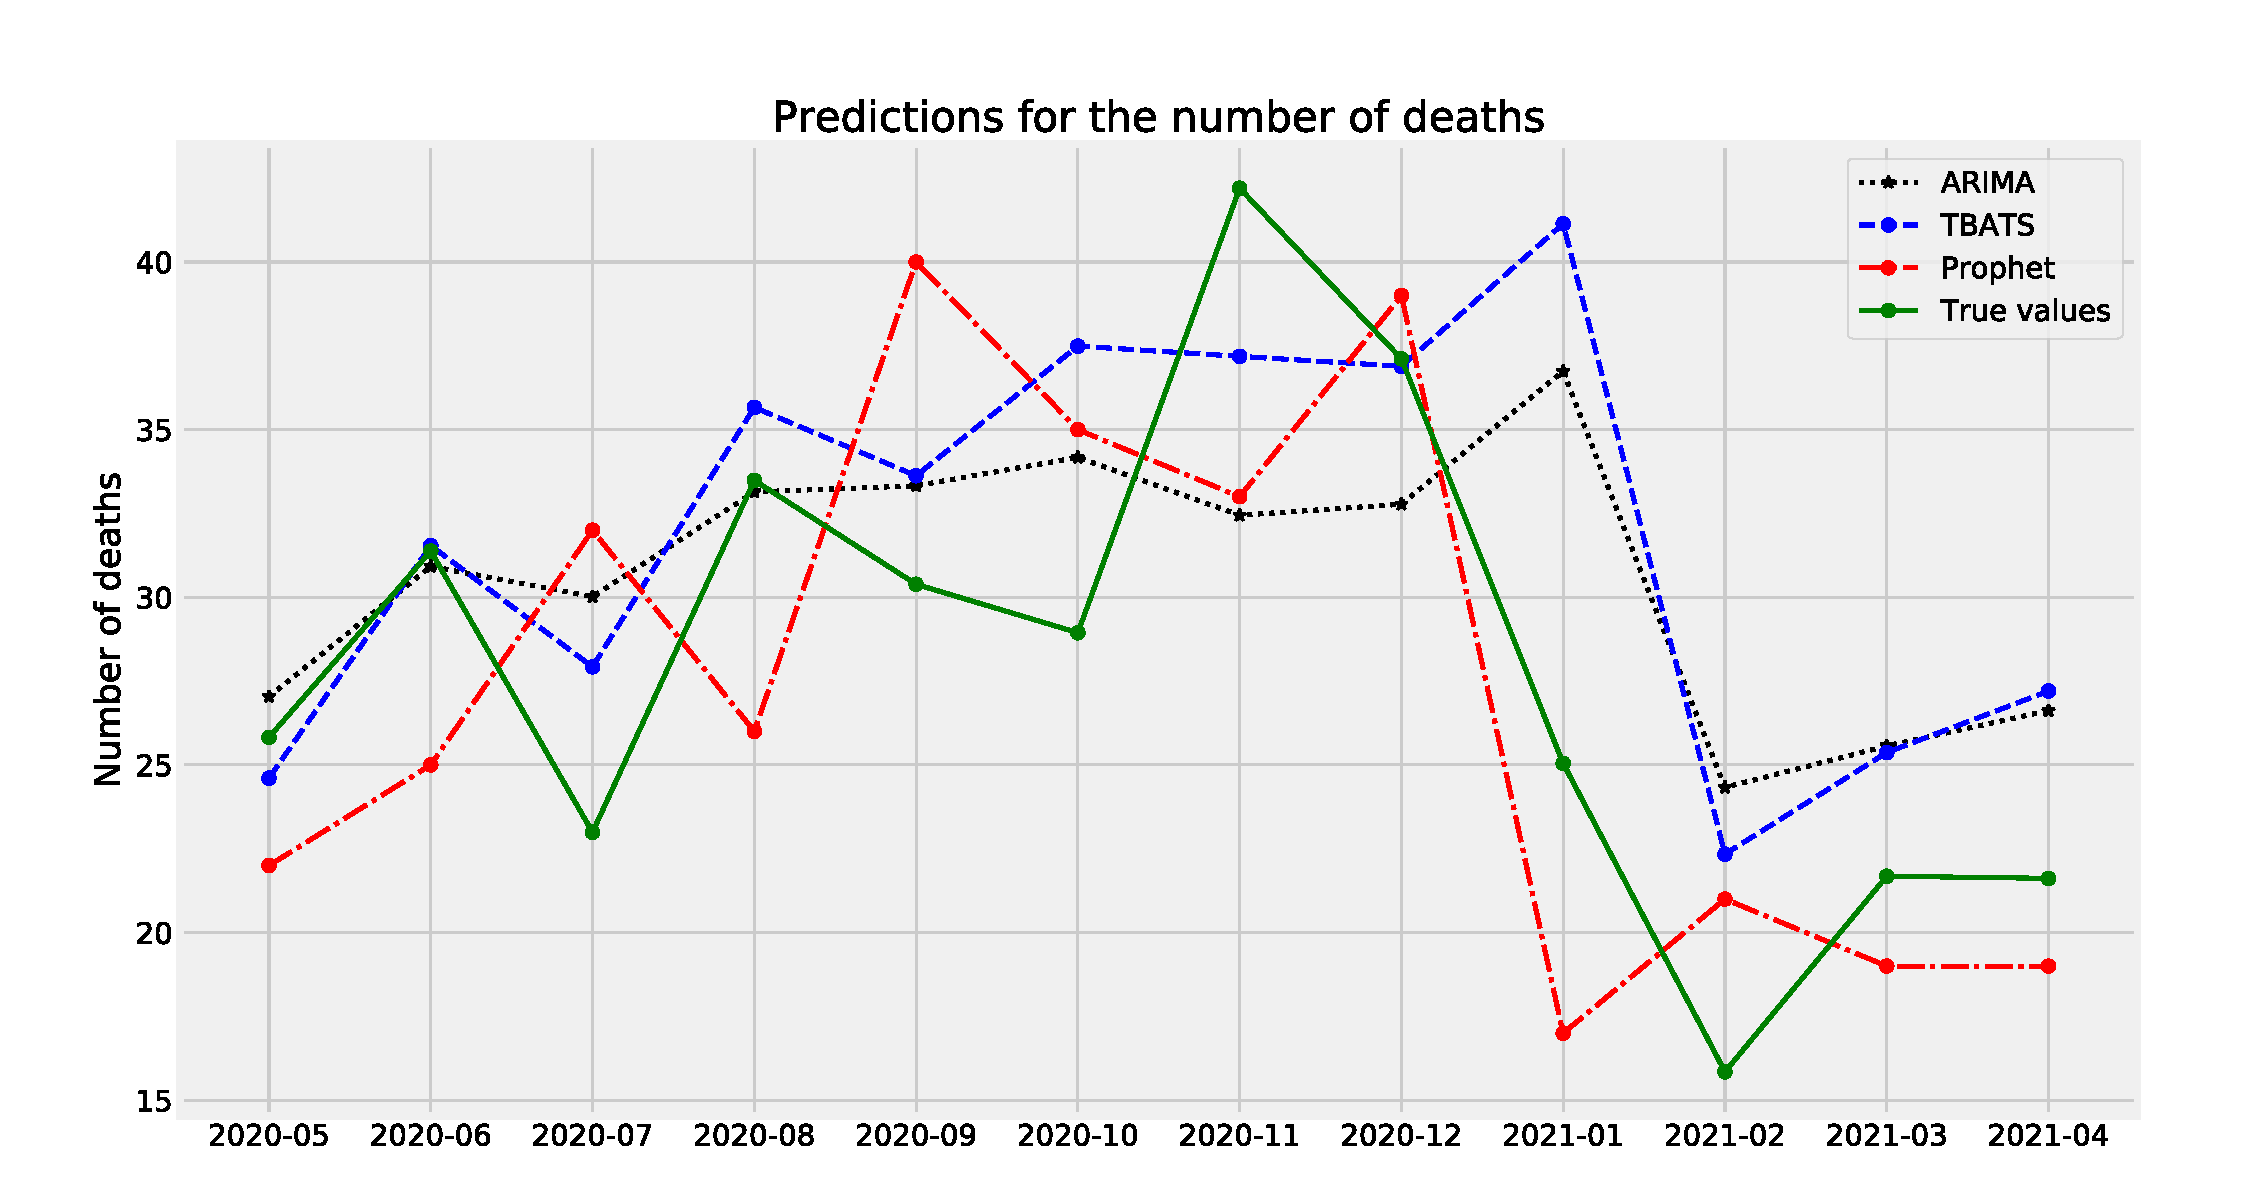
\includegraphics[width=0.8\textwidth]{../imgs/pdf_files/ts_predictions.pdf}
	\caption{\textbf{Time Series Death Predictions}}
	\label{fig:ts_predictions}
\end{figure}
\noindent
In order to meaningfully estimate the results of the two models we look at probabilities the models assign to each class
for every object and then compute metrics multiple times while changing the binarization threshold.
We can see that two models give comparable results with boosting performing slightly better. The results can be interpreted as follows.
As it was stated before two classes are heavily imbalanced, and they do overlap as well.
That highly influences precision of a minority class. It is very low.
The only pick of precision occurring while the threshold is low is attributed to the tiny sample of minority class objects
that the models are quite sure about, however this result cannot be interpreted as successful one due to recall being very low in this case. 
Low precision of minority class consequently influences metrics for imbalanced classification that we use. 
It is clear from the graphs, that both models are unable to give meaningful accuracy.
As authors think, it happens largely to the overlap of data.
That means that existing predictors are insufficient to accurately separate to classes.
Meaning that we actually really don’t have other valuable features, that may help us to predict the severity better. \\
In attempt to tackle that problem we fit models, specifically designed for imbalanced datasets.
Their results can be seen in the table.

\begin{table}[htpb]
	\centering
	\label{tab:metircs_imb}
	\resizebox{15cm}{!}
	{
\begin{tabular}{|c|c|c|c|c|c|c|c|}
	\hline
	 & \textbf{Cohen-Kappa} &	\textbf{MCC} & \textbf{AUC-Pr} & \textbf{Precision(Majority)} & \textbf{Precision(Minority)} & \textbf{Recall(Majority)} &	
 \textbf{Recall(Minority)} \\
	 \hline
		One-Class SVM & -0.025	& -0.05	& 0.044	& 0.938 &	0.036	& 0.491	& 0.371 \\
		\hline
		Isolation Forest & \textbf{0.054} & \textbf{0.054} &	\textbf{0.054}	& \textbf{0.954} &	\textbf{0.094}	& \textbf{0.039}	& 0.122 \\
		\hline
		Local Outlier Factor & 0.001 & 0.005 & \textbf{0.054} & 0.953 & 0.050	& 0.314	& \textbf{0.696} \\
		\hline
	\end{tabular}
}
\caption{\textbf{Imbalanced Classification Metrics}}
\end{table}
\noindent
As we can see these methods perform worse, with Isolation Forest giving slightly better results.
The reason for that may be the overlap as well.
And given the fact that all the methods are based on either drawing a hyperplane in object space or counting the distance
they cannot discriminate objects of two classes as those objects are very close to each other.

\section{Conclusion}
To conclude the whole research we can say, that overlapping data and imbalance significantly impeded the model construction.
Now let us review the dataset and draw meaningful summary of that work.

Firstly, exploratory data analysis clearly shows that, although the number of car crashes is at its height during the day,
one is less likely to end up being killed at noon. 
However, the chance of a tragic outcome increases almost fourfold at night.
Clustering car accidents also allows to obtain information on the most risky places.
Those places turn out to be junctions or motorways with a heavy traffic.

Secondly, the model for predicting the number of deaths in car accidents was constructed,
emulating the yearly seasonality and clear downward trend.
Based on comparison the best model turned out to be Prophet with Bayesian inference and MCMC simulations.

Thirdly, as we can see the existing data is insufficient to determine the outcome of a car accident.
It does not mean, that road or weather conditions have no influence on the outcome of a crash,
but that their impact is minor. At least there are other factors that are relevant and are not present in the dataset.
And that is actually true from the practical point of view.
The dataset has no information concerning the type of a vehicle, its conditions and safety equipment.
However, these things are highly important as they determine the extent to which driver is protected.
Moreover, we examined only the given features, but there is an option to construct some new features out of them.
For example one could create some combinations of features or use kernels to perform a non-linear transformation of given information.

So, based on the existing information it is impossible to meaningfully predict the outcome of a crash.
Therefore another research is needed to extract additional information and build a better model .


\cleardoublepage
\phantomsection
\addcontentsline{toc}{section}{References}
\begin{thebibliography}{99}
	\bibitem{Vision0}
	Matts-Ake Belina, Per Tillgrena, and Evert Vedungd, Vision Zero – a road safety policy innovation,
	\textit{International Journal of Injury Control and Safety Promotion}, \textbf{19}, No. 2, 171-179, 2012. 
	\bibitem{dtp_data}
	\href{https://dtp-stat.ru}
	{Проект <<Карта ДТП>>}
	\bibitem{DBSCAN}
	Ester, M., H. P. Kriegel, J. Sander, and X. Xu, A Density-Based Algorithm for Discovering Clusters in Large Spatial Databases with Noise,
	\textit{Proceedings of the 2nd International Conference on Knowledge Discovery and Data Mining}, 226-231, 1996.
	\bibitem{prophet}
	\href{https://peerj.com/preprints/3190.pdf}{Sean J. Taylor, Benjamin Letham, Forecasting at scale, \textit{The American Statistician}, (2018).}
	\bibitem{CKS}
	J. Cohen, A coefficient of agreement for nominal scales, \textit{Educational and Psychological measurement}, \textbf{20}, No. 1, (1960).
	\bibitem{MCC_intro}
	Matthews B. W., Comparison of the predicted and observed secondary structure of T4 phage lysozyme,
	\textit{Biochimica et Biophysica Acta (BBA) - Protein Structure}, \textbf{405}, 442–451, (1975).
	\bibitem{MCC_2000}
	P. Baldi, S. Brunak, Y. Chauvin, C. A. Andersen, H. Nielsen, Assessing the accuracy of prediction algorithms for classification:
	an overview, \textit{Bioinformatics}, \textbf{16}, No. 5, 412-424, 2000.
	\bibitem{MCC_new}
	D. Chicco, M. J. Warrens and G. Jurman, 
	The Matthews Correlation Coefficient (MCC) is More Informative Than Cohen’s Kappa and Brier Score in Binary Classification Assessment,
	\textit{IEEE Access}, \textbf{9}, 78368-78381, 2021.
	\bibitem{IsolForest}
	\href{https://cs.nju.edu.cn/zhouzh/zhouzh.files/publication/icdm08b.pdf}
	{Fei Tony Liu, Kai Ming Ting, Zhi-Hua Zhou, Isolation Forest, \textit{Data Mining}, 2008.}
	\bibitem{1SVM}
	\href{https://papers.nips.cc/paper/1999/file/8725fb777f25776ffa9076e44fcfd776-Paper.pdf}
	{Bernhard Scholkopf, Robert Williamson, Alex Smola, John Shawe-Taylort, John Platt, Support Vector Method for Novelty Detection,
	\textit{NIPS}, 1999.}
	\bibitem{LOF}
	Breunig, M. M., Kriegel, H. P., Ng, R. T., Sander, J, LOF: identifying density-based local outliers, \textit{ACM sigmod record}, 2000.
\end{thebibliography}

\end{document}
